\documentclass[11pt]{article}

\usepackage[utf8]{inputenc} % Para usar letras latinas acentuadas, como ãáà
\usepackage{verbatim}       % Para usar o comando \verb e o ambiente verbatim
\usepackage{hyperref}       % Links automáticos dentro do documento (e.g. citações, índice, ...)
                            % e links para a internet.
\usepackage{amsfonts}       % Tipos de letra matemáticos e comandos como \mathbb{R} e \mathcal{L}
\usepackage{amsmath}        % Símbolos matemáticos como \implies e \iff
\usepackage{float}          % Obrigar o LaTeX a pôr imagens/tabelas onde nós mandamos
\usepackage{graphicx}       % Incluir imagens no ambiente figure
\usepackage{xcolor}         % Para poderes escrever texto com outras cores
\usepackage{subcaption}     % Para o ambiente subfigure, que dispõe imagens lado a lado
\usepackage{listings}       % Inclusão de código
\usepackage{soulutf8}       % Para destacar texto com acentos


%%% Definir informações para a capa básica
\title{Intro LaTeX}
\author{Rodrigo Girão Serrão \\
        \href{mailto:rodrigogiraoserrao@gmail.com}{rodrigogiraoserrao@gmail.com}
}

%%% Definir o meu próprio comando com dois argumentos, #1 e #2
\newcommand{\partder}[2]{\frac{\partial #1}{\partial #2}}

%%% Definir um estilo para o código:
\definecolor{codegreen}{rgb}{0,0.6,0}
\definecolor{codegray}{rgb}{0.5,0.5,0.5}
\definecolor{codepurple}{rgb}{0.58,0,0.82}
\definecolor{backcolour}{rgb}{0.95,0.95,0.92}

\lstdefinestyle{mystyle}{
    backgroundcolor=\color{backcolour},   
    commentstyle=\color{codegreen},
    keywordstyle=\color{magenta},
    numberstyle=\tiny\color{codegray},
    stringstyle=\color{codepurple},
    basicstyle=\ttfamily\footnotesize,
    breakatwhitespace=false,         
    breaklines=true,                 
    captionpos=b,                    
    keepspaces=true,                 
    numbers=left,                    
    numbersep=5pt,                  
    showspaces=false,                
    showstringspaces=false,
    showtabs=false,                  
    tabsize=2
}
%%% Estilo definido

%%% "Figura" em vez de "Figure" nas legendas das imagens
\renewcommand{\figurename}{Figura}
\renewcommand{\refname}{Referências}

\begin{document}

\maketitle

\tableofcontents

\clearpage

\section{Introdução}

\subsection{Motivação}

O workshop ``Intro LaTeX'' foi criado com o objetivo de introduzir os alunos
da Licenciatura em Matemática Aplicada e Computação ao sistema LaTeX.
LaTeX é uma ferramenta útil para estes alunos porque, por um lado, há vários
trabalhos no curso que requerem a redação de um relatório e, por outro, porque
esses relatórios estão invariavelmente populados por várias fórmulas matemáticas
e outros objetos complexos.
É verdade que, com o passar do tempo, se tem tornado \textit{menos difícil} de
usar programas como o Microsoft Word para redigir documentos que contenham
fórmulas matemáticas e que sejam elegantes.
No entanto, LaTeX continua a ser a opção mais viável, de longe.

\subsection{Propósito deste documento}

Este documento tem dois propósitos:

\begin{enumerate}
    \item Primeiramente, serve como \textit{template} para os participantes do
    workshop e para todos os que queiram um documento simples com muitas
    funcionalidades demonstradas.

    \item Em segundo lugar, serve para me ajudar a ``mim'' (ou a qualquer outro
    palestrante) a dar o workshop de LaTeX.
\end{enumerate}

\clearpage
\section{Workshop}

\subsection{Conteúdo para iniciantes}

\paragraph{Criar um ficheiro \texttt{.tex}}

\paragraph{Preencher o cabeçalho com \texttt{\textbackslash documentclass\{article\}}}
Falar das configurações, e.g. mudar o tamanho do texto com \\
\verb|\documentclass[11pt]{article}|.

\paragraph{Explicar que o conteúdo do documento está entre
\texttt{\textbackslash begin\{document\}} e \texttt{\textbackslash end\{document\}}}

\paragraph{Explicar o que são ambientes}
Secções do documento em que o contexto é diferente e, por esse motivo, certas
coisas são interpretadas de forma especial.

\paragraph{Escrever uma frase e compilar}
Explicar que a compilação é o processo através do qual tudo o que escrevemos
é visto, interpretado e transformado num pdf (ou no que quer que seja).

\paragraph{Estilizar o texto com \texttt{textbf}, \texttt{textit} e \texttt{texttt}}
Os comandos começam com \texttt{text} e as duas letras seguintes indicam o tipo
de formatação:
\begin{itemize}
    \item \texttt{bf} para ``\textit{boldface}'', i.e. para \textbf{escrever texto
    em bold}.
    \item \texttt{it} para ``\textit{italics}'', i.e. para \textit{escrever texto
    em itálico}.
    \item \texttt{tt} para ``\textit{teletyperwriter}'', i.e. para \texttt{texto
    num tipo de letra com monoespaçamento}.
\end{itemize}

\paragraph{Explicar que os comandos aceitam argumentos dentro de \texttt{\{\}}}
Exemplo, \verb|\textbf{texto a bold}| produz \textbf{texto a bold}.

\paragraph{Falar do que são \textit{packages}}
Comandos que se põem no preâmbulo para adicionar funcionalidades. (Semelhante a
um \texttt{import *} em Python.)

\paragraph{Incluir a \textit{package} \texttt{inputenc} para lidar
com caracteres latinos, e.g. ãáà, com a opção \texttt{utf8}}

\paragraph{Falar de como mudar de linha}
\begin{itemize}
    \item uma quebra de linha é para escrever linhas mais curtas;
    \item duas quebras de linha consecutivas mudam o texto de linha;
    \item escrever \verb|\\| também muda de linha;
    \item usar \verb|\newline| para mudar de linha;
    \item usar \verb|\vspace{length}| para espaço vertical arbitrário.
\end{itemize}

Por exemplo, esta frase foi escrita
em duas linhas diferentes do documento físico.

Por outro lado, esta tem uma linha branca vazia a separá-la da linha de cima.
Também temos que \textbackslash\textbackslash~faz com \\ que o texto mude de linha.

Para concluir, para conseguir que este texto ficasse tão afastado
\vspace{3em}
do resto da frase, tivémos de usar o comando \verb|\vspace{3em}|.

\paragraph{Explicar que \$ e \$\$ são usados para ``escrever matemática''}
Explicar que \$ é usado para números/fórmulas que ficam corridos com o texto,
por exemplo para mostrar que ``x mais dois'' fica $x+2$, e dizer que \$\$
é usado para rodear expressões a que queremos dar destaque, tais como

$$x + 3 ~.$$

\paragraph{Mencionar o site
\href{https://detexify.kirelabs.org}{detexify.kirelabs.org}}

Site onde desenhamos os sím-bolos e eles dão-nos o comando.

\paragraph{\textit{Package} \texttt{amsfonts} para os comandos
\texttt{mathbb} e \texttt{mathcal}}
\verb|\mathbb{R}| é usado para produzir o símbolo dos números reais $\mathbb{R}$
e \verb|\mathcal{L}| produz letras caligrafadas: $\mathcal{L}$.

\paragraph{\textit{Package} \texttt{amsmath} para comandos como \texttt{implies}}
\verb|\implies| é usado para $\implies$.

\paragraph{Mostrar uma série de símbolos comuns}
Olhar para a tabela que se segue.

\begin{table}[H]
    \centering
    \caption{Alguns símbolos e comandos respetivos (muitos precisam de
    \texttt{amsfonts} ou \texttt{amsmath})}
    \begin{tabular}{|l|l|l|l|} \hline
        \textbf{Símb.} & \textbf{Comando} &
        \textbf{Símb.} & \textbf{Comando} \\\hline
        $\mathbb{C}$ & \verb|\mathbb{C}| &
        $\mathbb{R}$ & \verb|\mathbb{R}| \\\hline
        $\mathbb{Q}$ & \verb|\mathbb{Q}| &
        $\mathbb{Z}$ & \verb|\mathbb{Z}| \\\hline
        $\mathbb{N}$ & \verb|\mathbb{N}| &
        $\implies$ & \verb|\implies| \\\hline
        $\iff$ & \verb|\iff| &
        $\equiv$ & \verb|\equiv| \\\hline
        $\approx$ & \verb|\approx| &
        $\neq$ & \verb|\neq| \\\hline
        $\lim$ & \verb|\lim| &
        $\sum$ & \verb|\sum| \\\hline
        $\prod$ & \verb|\prod| &
        $\int$ & \verb|\int| \\\hline
        $\alpha$ & \verb|\alpha| &
        $\pi$ & \verb|\pi| \\\hline
        $\phi$ & \verb|\phi| &
        $\Phi$ & \verb|\Phi| \\\hline
        $\to$ & \verb|\to| &
        $\infty$ & \verb|\infty| \\\hline
        $\leq$ & \verb|\leq| &
        $\geq$ & \verb|\geq| \\\hline
    \end{tabular}
\end{table}

\paragraph{Comando \texttt{sqrt} para raízes quadradas}
Usar \verb|\sqrt{3\pi - \infty}| dá $\sqrt{3\pi - \infty}$.

\paragraph{Falar do ambiente \texttt{equation}}
Centra as equações e numera-as automaticamente. Por exemplo, ``x mais dois''

\begin{equation}
    x + 2
\end{equation}

\paragraph{Explicar como impedir numeração em geral com *}
Por exemplo, \verb|\begin{equation*} ... \end{equation*}| cria uma equação
sem número:

\begin{equation*}
    x + 3
\end{equation*}

\paragraph{Ensinar a usar \texttt{\^} para potências e similares,
e \texttt{\_} para índices e similares}
Mostrar $x^2$ e $v_i$.

\paragraph{Ensinar \texttt{\{\}} para agrupar várias coisas agarradas a
\texttt{\^} ou \texttt{\_}}
Por exemplo, \verb|\lim_{x \to \infty} f(x)| cria
$$\lim_{x \to \infty} f(x)$$
e \verb|\int_0^{2\pi + \pi^2} f(x)dx| cria
$$\int_0^{2\pi + \pi^2} f(x)~dx$$

\paragraph{Ensinar frações}
\verb|\frac{num}{den}| produz $\frac{num}{den}$.

\paragraph{Alinhar equações com o ambiente \texttt{align}}
Usamos \& para indicar o ponto de alinhamento e usamos \textbackslash\textbackslash~
para dizer que mudámos de linha. Por exemplo,
\begin{align}
    x &= 1 + \pi \\
    y &= 0
\end{align}
foi produzido com
\begin{verbatim}
    \begin{align}
        x &= 1 + \pi \\
        y &= 0
    \end{align}
\end{verbatim}

\paragraph{Agrupar equações com o sub-ambiente \texttt{cases}}
Usamos \textbackslash\textbackslash~para dizer que mudámos de linha. Por exemplo,
\begin{equation}
    f(x) = \begin{cases}
        0, x < 0 \\
        1, x \geq 0
    \end{cases}
\end{equation}
foi produzido com
\begin{verbatim}
    \begin{equation}
        f(x) = \begin{cases}
            0, x < 0 \\
            1, x \geq 0
        \end{cases}
    \end{equation}
\end{verbatim}

\paragraph{Obrigar o LaTeX a pôr espaços onde queremos com \textasciitilde}
Por exemplo, para pôr um espaço na equação em cima entre a vírgula e as condições:
\begin{equation}
    f(x) = \begin{cases}
        0, ~ x < 0 \\
        1, ~ x \geq 0
    \end{cases}
\end{equation}
foi produzido com
\begin{verbatim}
    \begin{equation}
        f(x) = \begin{cases}
            0, ~ x < 0 \\
            1, ~ x \geq 0
        \end{cases}
    \end{equation}
\end{verbatim}

\paragraph{Escrever texto dentro de ambientes matemáticos com \texttt{text}}
Por exemplo, a segunda condição em cima podia ser
\begin{equation}
    f(x) = \begin{cases}
        0, ~ x < 0 \\
        1, ~ \text{c.c.}
    \end{cases}
\end{equation}
que foi produzido com
\begin{verbatim}
    \begin{equation}
        f(x) = \begin{cases}
            0, ~ x < 0 \\
            1, ~ \text{c.c.}
        \end{cases}
    \end{equation}
\end{verbatim}

\paragraph{Ter cuidado com o estilo com que se escreve LaTeX}
Escrever à badalhoco é meio caminho andado para se escrever um documento impossível
de editar posteriormente.

\paragraph{Funções trigonométricas et al, com os próprios nomes}
Certas fun-ções e/ou símbolos existem como comandos com o próprio nome, por exemplo
\verb|\sin(\pi)|, \verb|\min(0, 1)| e \verb|\gcd(1, 2)| para
$\sin(\pi)$, $\min(0, 1)$ e $\gcd(1, 2)$

\paragraph{Tamanho vertical de parêntesis com \texttt{left} e \texttt{right}}
Se expressões dentro de parêntesis (ou entre dois delimitadores, em geral)
ficarem muito altas, podemos usar \verb|\left| e \verb|\right| para acertar
o tamanho vertical. Compare-se, por exemplo,
$$\sin(\sum_0^\infty x_n) ~ \text{vs} ~ \sin\left( \sum_0^\infty x_n \right)$$
que foi escrito com
\begin{verbatim}
\sin(\sum_0^\infty x_n) ~ \text{vs} ~ 
    \sin\left( \sum_0^\infty x_n \right)
\end{verbatim}

\paragraph{Usar etiquetas (\texttt{label}) para nos referirmos a outros objetos}
Todos os objetos que são numerados podem ser referenciados. Para tal, escolher
um nome que identifique \textit{claramente} esse objeto e pôr esse nome dentro
do comando \verb|\label|. Mais tarde, fazer referência ao objeto através do
comando \verb|\ref| que aceita o nome da etiqueta como argumento.

Por exemplo, o código
\begin{verbatim}
    \begin{equation}
        \label{eq:quadratic_formula}
        x = \frac{-b \pm \sqrt{b^2 - 4ac}}{2a}
    \end{equation}
\end{verbatim}
produz a equação:
\begin{equation}
    \label{eq:quadratic_formula}
    x = \frac{-b \pm \sqrt{b^2 - 4ac}}{2a}
\end{equation}
e agora podemos falar especificamente da equação \ref{eq:quadratic_formula},
através da utilização do comando \verb|\ref{eq:quadratic_formula}|. Para fórmulas,
também fica bem usar o comando \verb|\eqref{eq:quadratic_formula}|, que tem um
estilo ligeiramente diferente, para podermos falar da equação
\eqref{eq:quadratic_formula}.

\paragraph{Usar prefixos nas etiquetas para agrupar objetos da mesma família}
Por exemplo, \texttt{eq:} para equações, \texttt{fig:} ou \texttt{img:} para imagens,
\texttt{t:} ou \texttt{tab:} para tabelas, \texttt{sec:} para secções
e \texttt{subsec:} para subsecções, etc. Ser \textbf{consistente}.

\paragraph{Usar \texttt{section}, \texttt{subsection} e \texttt{subsubsection}}
Estes comandos partem o documento em secções, subsecções e sub-subsecções.
A numeração é automática. O único argumento é o nome da divisão. Por exemplo, o
código
\begin{verbatim}
    \section{Introdução
    \subsection{Motivação}
    \subsection{Propósito deste documento}
    \section{Workshop}
    \subsection{Conteúdo para iniciantes}
    \subsection{Conteúdo intermédio}
    \subsection{Conteúdo avançado}
\end{verbatim}
foi usado para separar este documento nas partes que se encontram no índice.

\paragraph{Criar um índice com \texttt{tableofcontents}}
Basta usar o comando \verb|\tableofcontents| no sítio em que queremos o índice.

\paragraph{Criar uma capa com \texttt{maketitle}}
Especificar informações como \texttt{author} e \texttt{title} no preâmbulo,
e.g. com
\begin{verbatim}
    \title{Intro LaTeX}
    \author{Rodrigo Girão Serrão \\
            rodrigogiraoserrao@gmail.com
    }
\end{verbatim}
e depois incluir a capa com \verb|\maketitle|

\paragraph{Obrigar o resto da página a ficar em branco com \texttt{clearpage}}
Por exemplo, quando queremos que o índice não seja logo seguido de texto, usamos
\verb|\clearpage|, por isso é que há tanto espaço em branco na primeira página deste
documento, porque o documento começa (mais ou menos) com
\begin{verbatim}
    \begin{document}
    \maketitle
    \tableofcontents
    \clearpage
    \section{Introdução}
    \subsection{Motivação}
    ...
\end{verbatim}

\paragraph{Incluir imagens com \texttt{graphicx}}
O pacote \texttt{graphicx} dá-nos acesso a um ambiente \texttt{figure} que usamos
para incluir imagens. Se tivermos uma imagem no caminho \texttt{graphics/image.png},
podemos incluí-la, centrá-la e mudar o seu tamanho com
\begin{verbatim}
    \begin{figure}
        \centering
        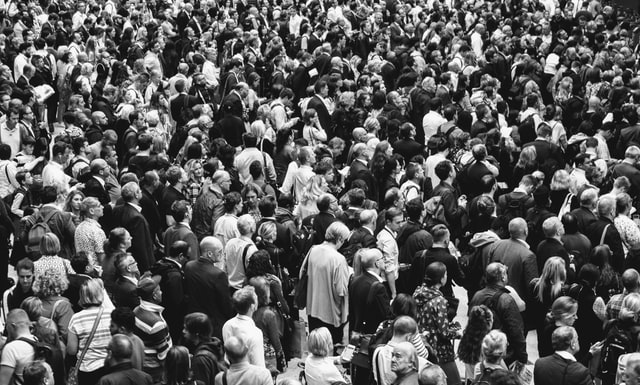
\includegraphics[scale=0.3]{graphics/crowd.jpg}
        \caption{Legenda da imagem}
        \label{img:first-example}
    \end{figure}
\end{verbatim}
que produz a imagem \ref{img:first-example}.

\begin{figure}
    \centering
    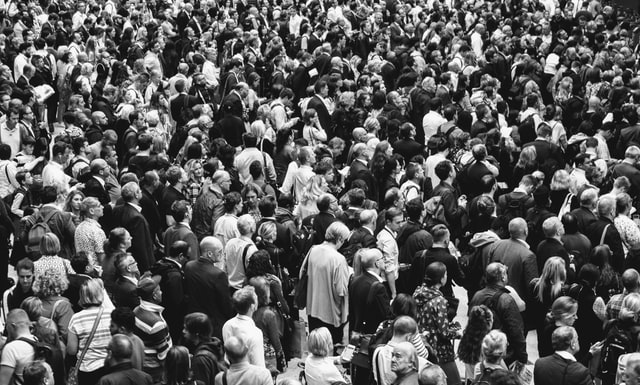
\includegraphics[scale=0.3]{graphics/crowd.jpg}
    \caption{Legenda da imagem}
    \label{img:first-example}
\end{figure}

\paragraph{A etiqueta tem de vir depois da legenda}
É a legenda que atribui o número à imagem, logo convém haver um número para lhe
podermos atribuir uma etiqueta.

\paragraph{A opção \texttt{scale} rescala a imagem de forma proporcionada}

\paragraph{Alternativamente, a opção \texttt{width} com
\texttt{\textbackslash linewidth} especifica o comprimento}

\paragraph{Usar o pacote \texttt{float} para obrigar a imagem a ficar no lugar}
Abrindo o ambiente com \verb|\begin{figure}[H]| obriga a imagem a ficar
no sítio onde foi definida. Por exemplo, a imagem está aqui:

\begin{figure}[H]
    \centering
    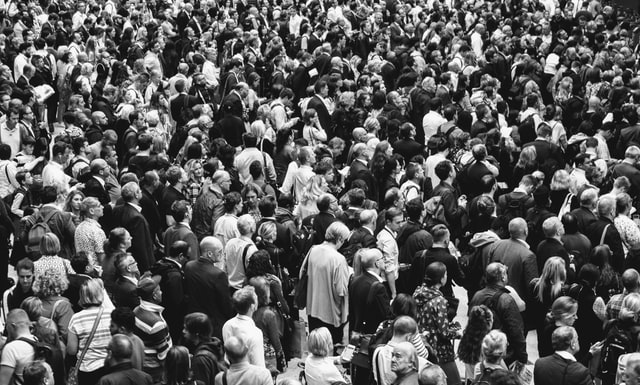
\includegraphics[width=0.5\linewidth]{graphics/crowd.jpg}
    \caption{Legenda da imagem}
    \label{img:second-example}
\end{figure}
graças ao código (depois de pôr \verb|\usepackage{float}| no preâmbulo)
\begin{verbatim}
    \begin{figure}[H]
        \centering
        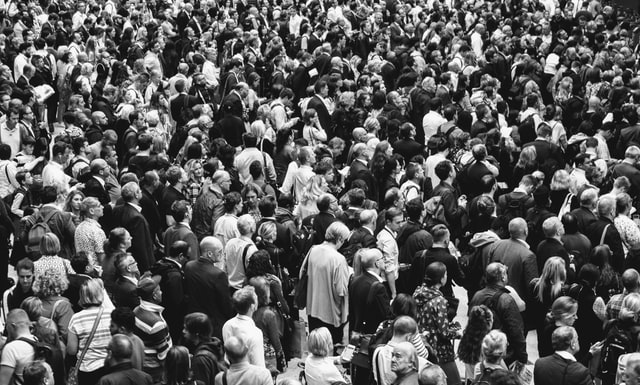
\includegraphics[width=0.5\linewidth]{graphics/crowd.jpg}
        \caption{Legenda da imagem}
        \label{img:second-example}
    \end{figure}
\end{verbatim}

\paragraph{Bibliografia básica}
Usar o ambiente \\ \verb|\begin{thebibliography}{99} ... \end{thebibliograph}|.
Dentro do ambiente, cada linha que comece com \verb|\bibitem{lbl}| é uma entrada.
\texttt{lbl} é um nome de etiqueta para citarmos a bibliografia. Por exemplo,
a bibliografia
\begin{thebibliography}{99}
    \bibitem{wiki} Wikipedia, lol
    \bibitem{site} Outro site qualquer
\end{thebibliography}
foi inserida com
\begin{verbatim}
    \begin{thebibliography}[99]
        \bibitem{wiki} Wikipedia, lol
        \bibitem{site} Outro site qualquer
    \end{thebibliography}
\end{verbatim}
(e com uma batota no preâmbulo para ter o nome em português).

\paragraph{Citar a bibliografia com \texttt{cite}}
Eu sei isto, cf. \cite{wiki}! (\verb|\cite{wiki}| para a citação).

\paragraph{Links no próprio pdf com \texttt{hyperref}}
Usar o pacote \texttt{hyperref} faz com que citações e referências sejam
clicáveis (bem como o índice) e permitem-nos ir diretamente para o objeto
referido.

\paragraph{Links externos com \texttt{href}}
O comando \verb|\href{url}{text}| cria links externos, e.g. para a internet,
com texto personalizado e \verb|\url{url}| cria links, e.g.
\href{https://google.com}{este link vai para o Google}, e este também:
\url{https://google.com}.
\verb|\href{https://google.com}{este link vai para o Google}| vs.
\verb|\url{https://google.com}|

\paragraph{Listas}
Usar o ambiente \texttt{itemize} e comando \texttt{item} para fazer uma lista não ordenada.
A lista

\begin{itemize}
    \item Item 1
    \item Item 2
    \item Item 3
\end{itemize}

cria-se com o código

\begin{verbatim}
    \begin{itemize}
        \item Item 1
        \item Item 2
        \item Item 3
    \end{itemize}
\end{verbatim}

\paragraph{Listas dentro de listas}
Usar um ambiente \texttt{itemize} dentro de um \texttt{item} cria outra lista.
De facto, a lista

\begin{itemize}
    \item Item 1 \begin{itemize}
        \item Sub 1
        \item Sub 2
    \end{itemize}
    \item Item 2
    \item Item 3 \begin{itemize}
        \item Outro Sub 1
        \item Outro Sub 2
    \end{itemize}
\end{itemize}

é criada com o código

\begin{verbatim}
    \begin{itemize}
        \item Item 1 \begin{itemize}
            \item Sub 1
            \item Sub 2
        \end{itemize}
        \item Item 2
        \item Item 3 \begin{itemize}
            \item Outro Sub 1
            \item Outro Sub 2
        \end{itemize}
    \end{itemize}
\end{verbatim}

\paragraph{Enumerações}
O ambiente \texttt{enumerate} é semelhante ao \texttt{itemize},
mas serve para listas ordenadas.
Se pegarmos no código em cima e trocarmos todos os \texttt{itemize}
por \texttt{enumerate}, obtemos o seguinte:

\begin{enumerate}
    \item Item 1 \begin{enumerate}
        \item Sub 1
        \item Sub 2
    \end{enumerate}
    \item Item 2
    \item Item 3 \begin{enumerate}
        \item Outro Sub 1
        \item Outro Sub 2
    \end{enumerate}
\end{enumerate}

\paragraph{Tabelas}
Ambiente \texttt{table}.
Tal como com as imagens, podes usar \texttt{centering} e
\texttt{[H]} para centrar e pôr a tabela onde a escreveste.
Dentro do \texttt{table}, ambiente \texttt{tabular} é usado para escrever os
dados, separados por \& e o argumento do \texttt{tabular} é uma sequência de letras
\texttt{lcr} para indicar se cada coluna é alinhada à esquerda, ao centro ou à
direita, respetivamente. (Há tantas letras quanto colunas.)
O código
\begin{verbatim}
    \begin{table}[H]
        \centering
        \begin{tabular}{lccr}
            um & dois & três & $3 + 3 + \pi$ \\
            1 & 2 & 3 & três mais três mais pi
        \end{tabular}
        \caption{Tabela básica}
    \end{table}
\end{verbatim}
produz a tabela
\begin{table}[H]
    \centering
    \begin{tabular}{lccr}
        um & dois & três & $3 + 3 + \pi$ \\
        1 & 2 & 3 & três mais três mais pi
    \end{tabular}
    \caption{Tabela básica}
\end{table}

\paragraph{Usa \textbar~cenas para linhas verticais na tabela}
O código
\begin{verbatim}
    \begin{table}[H]
        \centering
        \begin{tabular}{|l|cc|r}
            um & dois & três & $3 + 3 + \pi$ \\
            1 & 2 & 3 & três mais três mais pi
        \end{tabular}
        \caption{Tabela básica}
    \end{table}
\end{verbatim}
produz a tabela
\begin{table}[H]
    \centering
    \begin{tabular}{|l|cc|r}
        um & dois & três & $3 + 3 + \pi$ \\
        1 & 2 & 3 & três mais três mais pi
    \end{tabular}
    \caption{Tabela básica}
\end{table}

\paragraph{Usa \texttt{hline} para linhas horizontais na tabela}
O código
\begin{verbatim}
    \begin{table}[H]
        \centering
        \begin{tabular}{|l|cc|r}
            \hline
            um & dois & três & $3 + 3 + \pi$ \\
            \hline
            1 & 2 & 3 & três mais três mais pi \\
            \hline
        \end{tabular}
        \caption{Tabela básica}
    \end{table}
\end{verbatim}
produz a tabela
\begin{table}[H]
    \centering
    \begin{tabular}{|l|cc|r}
        \hline
        um & dois & três & $3 + 3 + \pi$ \\
        \hline
        1 & 2 & 3 & três mais três mais pi \\
        \hline
    \end{tabular}
    \caption{Tabela básica}
\end{table}

\paragraph{Usa \url{https://tablesgenerator.com} para gerar tabelas mais facilmente}

\paragraph{Cria matrizes com ambientes como \texttt{bmatrix} e \texttt{pmatrix}}
O ambiente exato altera o aspeto dos parêntesis à volta da matriz.
Separamos os elementos numa linha com \& e separamos linhas com
\textbackslash\textbackslash.
Exemplo:
$$
\begin{bmatrix} 1 & 0 \\ 0 & 1 \end{bmatrix}^{-1} = 
\begin{pmatrix} 1 & 0 \\ 0 & 1 \end{pmatrix}
$$
Produzido com o código
\begin{verbatim}
    $$
    \begin{bmatrix} 1 & 0 \\ 0 & 1 \end{bmatrix}^{-1} = 
    \begin{pmatrix} 1 & 0 \\ 0 & 1 \end{pmatrix}
    $$
\end{verbatim}

\paragraph{As linhas da matriz podem, e devem, estar em linhas separadas}
Por exemplo, a matriz
$$ \begin{bmatrix}
    1 & 2 & 3 & 4 \\
    \pi & 2\pi & 3\pi & 4\pi \\
    5 & 6 & 7 & 8
\end{bmatrix} $$
(não é invertível e) foi produzida com o código
\begin{verbatim}
    $$ \begin{bmatrix}
        1 & 2 & 3 & 4 \\
        \pi & 2\pi & 3\pi & 4\pi \\
        5 & 6 & 7 & 8
    \end{bmatrix} $$
\end{verbatim}

\paragraph{Cria matrizes online em \url{https://codecogs.com/latex/eqneditor.php}}
Ou edita qualquer tipo de equação lá.

\paragraph{Cria links para equações em \url{https://mathspp.com/texpaste}}
Para partilhares equações diretamente em qualquer meio,
para que o utilizador não tenha de tentar decifrar o código LaTeX.
Por exemplo, \href{https://mathspp.com/texpaste\#0U1GpULBViEkrSkyu1k1SiCnIVYgpLiwqqU6KM1LQVTBJTK6trTZKrFVRAQA}
{este link} mostra a solução de uma equação quadrática.

\subsection{Conteúdo intermédio}
A partir daqui estamos a aprender funcionalidades que um utilizador intermédio
de LaTeX usaria.

\paragraph{Incluir código com o pacote \texttt{listings}}
Usar o ambiente \texttt{lstlisting}. Por exemplo:
\begin{lstlisting}[language=Python]
if __name__ == "__main__":
    print("Hello, World!")
\end{lstlisting}
é gerado com
\begin{verbatim}
    \begin{lstlisting}[language=Python]
        if __name__ == "__main__":
            print("Hello, World!")
    \end{lstlisting}
\end{verbatim}

\paragraph{Incluir código diretamente de um ficheiro com \texttt{lstinputlisting}}
Por exemplo, se o ficheiro \texttt{pythoncode.py} estiver no mesmo diretório que
este ficheiro \texttt{.tex}, então o comando \\
\verb|\lstinputlisting[language=Python]{pythoncode.py}| produz:

\lstinputlisting[language=Python]{pythoncode.py}

\paragraph{Pesquisar online por estilos pré-definidos para usar com código}
Por exemplo, no preâmbulo deste documento defini um estilo \texttt{mystyle} e agora
o comando \\
\verb|\lstinputlisting[language=Python,style=mystyle]{pythoncode.py}| \\
produz

\lstinputlisting[language=Python,style=mystyle]{pythoncode.py}

Continua feio, mas está \textit{muito} melhor.

\paragraph{Comando \texttt{lstinline} para código em texto corrido}
A utilização do comando
\begin{verbatim}
    \lstinline[language=Python,style=mystyle]
    {if __name__ == "__main__": print("Hey")}
\end{verbatim}
permite-me escrever
\lstinline[language=Python,style=mystyle]{if __name__ == "__main__": print("Hey")}.

\paragraph{Alinhamento múltiplo com \texttt{alignat}}
Para produzir uma equação com vários alinhamentos (2 ou mais) como a seguinte,
usa-se o ambiente \texttt{alignat}, cujo argumento é o número de alinhamentos
verticais.
O primeiro alinhamento de cada linha faz-se com \& e os seguintes com \&\&.
\begin{alignat}{2}
    \mathcal{L}u &= f, ~ &&\text{in} ~ \Omega \\
    u &= g + g^2, ~ &&\text{on} ~ \partial\Omega
\end{alignat}
produzido com
\begin{verbatim}
    \begin{alignat}{2}
        \mathcal{L}u &= f, ~ &&\text{in} ~ \Omega \\
        u &= g + g^2, ~ &&\text{on} ~ \partial\Omega
    \end{alignat}
\end{verbatim}

\paragraph{Alinhamento múltiplo dentro de outros ambientes com \texttt{aligned}}
A equação
$$ u ~ \text{solves} ~
\begin{cases}
    \begin{aligned}
        \mathcal{L}u &= f, ~ &&\text{in} ~ \Omega \\
        u &= g + g^2, ~ &&\text{on} ~ \partial\Omega
    \end{aligned}
\end{cases} $$
foi produzida com o código
\begin{verbatim}
    $$ u ~ \text{solves} ~
    \begin{cases}
        \begin{aligned}
            \mathcal{L}u &= f, ~ &&\text{in} ~ \Omega \\
            u &= g + g^2, ~ &&\text{on} ~ \partial\Omega
        \end{aligned}
    \end{cases} $$
\end{verbatim}

\paragraph{Figuras lado a lado com \texttt{subcaption}}
Usar o pacote \texttt{subcaption} dá acesso ao ambiente \texttt{subfigure},
que permite pôr imagens lado a lado.
O ambiente aceita um argumento que é o espaço horizontal a usar.
\begin{figure}[H]
    \centering
    \begin{subfigure}{0.49\textwidth}
        \centering
        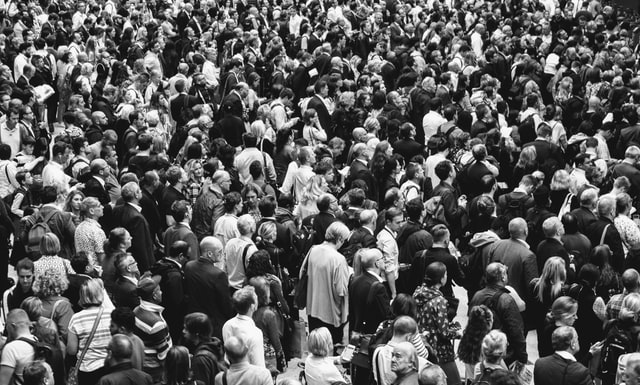
\includegraphics[width=0.99\textwidth]{graphics/crowd.jpg}
        \caption{
            Sub 1 tem imenso texto aqui
            que obviamente não cabe numa só linha
        }
        \label{fig:sub1}
    \end{subfigure}
    \begin{subfigure}{0.49\textwidth}
        \centering
        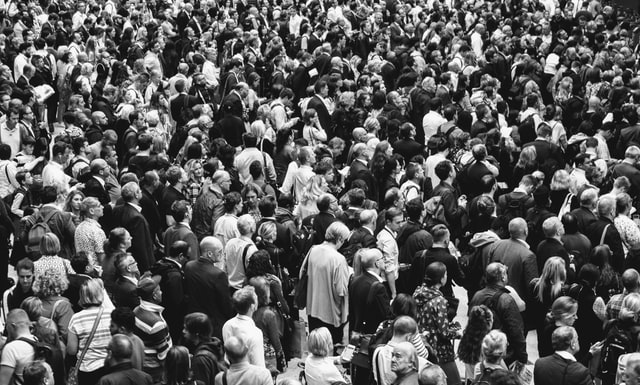
\includegraphics[height=4em]{graphics/crowd.jpg}
        \caption{Sub 2}
        \label{fig:sub2}
    \end{subfigure}
    \caption{Legenda principal}
    \label{fig:big-figure}
\end{figure}
Podemos falar da figura toda com \ref{fig:big-figure} ou das sub-imagens com
\ref{fig:sub1} e \ref{fig:sub2}.
O código para pôr as imagens é
\begin{verbatim}
    \begin{figure}[H]
        \centering
        \begin{subfigure}{0.49\textwidth}
            \centering
            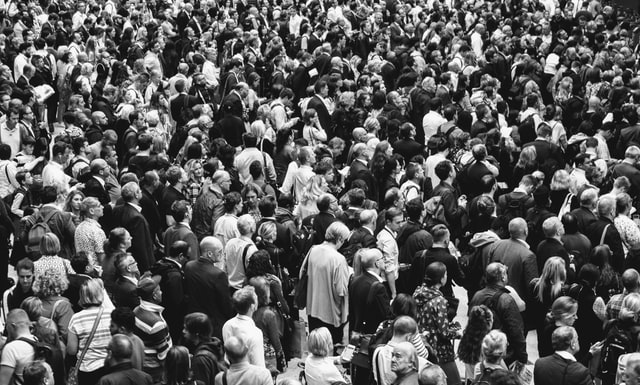
\includegraphics[width=0.99\textwidth]{graphics/crowd.jpg}
            \caption{
                Sub 1 tem imenso texto aqui
                que obviamente não cabe numa só linha
            }
            \label{fig:sub1}
        \end{subfigure}
        \begin{subfigure}{0.49\textwidth}
            \centering
            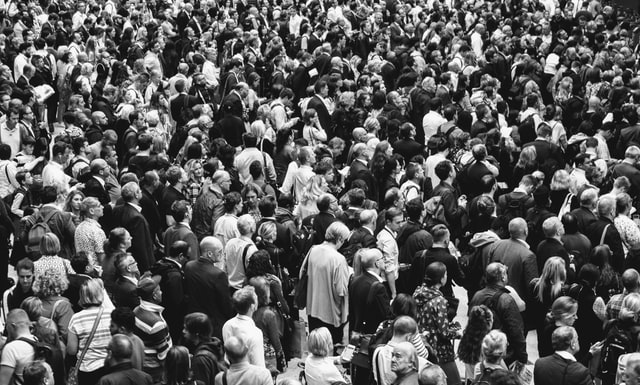
\includegraphics[height=4em]{graphics/crowd.jpg}
            \caption{Sub 2}
            \label{fig:sub2}
        \end{subfigure}
        \caption{Legenda principal}
        \label{fig:big-figure}
    \end{figure}
\end{verbatim}
e para as referir é \verb|\ref{fig:big-figure}| ou \verb|\ref{fig:sub2}|, por exemplo.

\paragraph{Alinhar as sub-legendas com \texttt{[b]} ou \texttt{[t]}}
Opções para o ambiente \texttt{subfigure}. Alinhas pelo \textit{top} ou
\textit{bottom} das legendas.
Efeito (imagens mais pequenas para ocuparem menos espaço):
\begin{figure}[H]
    \centering
    \begin{subfigure}[t]{0.49\textwidth}
        \centering
        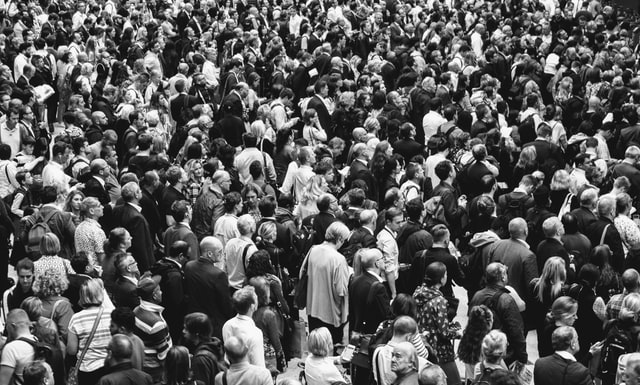
\includegraphics[height=3em]{graphics/crowd.jpg}
        \caption{Sub 1 tem imenso texto aqui que obviamente não cabe numa só linha}
        \label{fig:sub1}
    \end{subfigure}
    \begin{subfigure}[t]{0.49\textwidth}
        \centering
        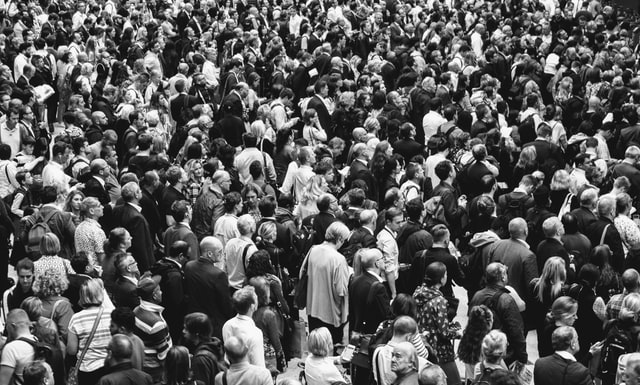
\includegraphics[height=4em]{graphics/crowd.jpg}
        \caption{Sub 2}
        \label{fig:sub2}
    \end{subfigure}
    \caption{\texttt{\textbackslash begin{subfigure}[t] ...}}
    \label{fig:big-figure}
\end{figure}
e
\begin{figure}[H]
    \centering
    \begin{subfigure}[b]{0.49\textwidth}
        \centering
        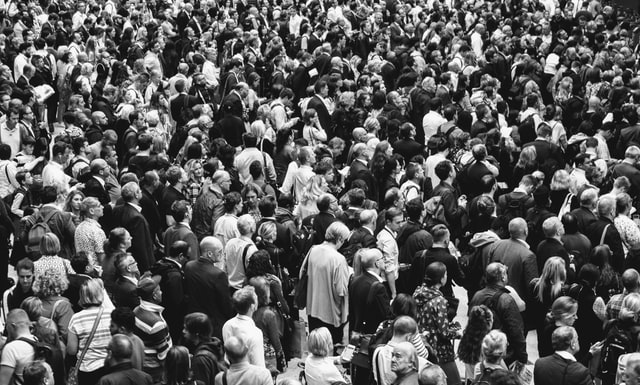
\includegraphics[height=3em]{graphics/crowd.jpg}
        \caption{Sub 1 tem imenso texto aqui que obviamente não cabe numa só linha}
        \label{fig:sub1}
    \end{subfigure}
    \begin{subfigure}[b]{0.49\textwidth}
        \centering
        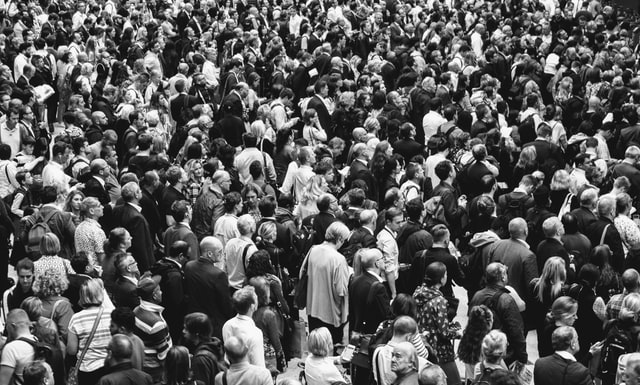
\includegraphics[height=4em]{graphics/crowd.jpg}
        \caption{Sub 2}
        \label{fig:sub2}
    \end{subfigure}
    \caption{\texttt{\textbackslash begin{subfigure}[b] ...}}
    \label{fig:big-figure}
\end{figure}

\paragraph{Criar os próprios comandos com \texttt{newcommand}}
Definem-se no preâmbulo e a sintaxe é
\verb|\newcommand{\cmdname}[nargs]{syntax}|
onde \texttt{nargs} é o número de argumentos que o comando aceita,
e para nos referirmos a esses argumentos usamos \verb|#1|, \verb|#2|, etc.

Por exemplo, inserir \\
\verb|\newcommand{\partder}[2]{\frac{\partial #1}{\partial #2}}|
no \\ preâmbulo permite que o código \verb|$\partder{f}{x}$| gere $\partder{f}{x}$.

\paragraph{Criar um apêncide com \texttt{appendix}}
Se usarmos o comando \verb|\appendix|, a partir daí todas as secções, subsecções, etc,
ficam identificadas como pertencendo ao apêndice e numeradas de forma diferente.
Vejam, por exemplo, a secção \ref{sec:first-sec-in-appendix}.

\paragraph{Ignorar caracteres especiais com \textbackslash}
Há vários caracteres que são especiais. Usamos \textbackslash~
para os ignorar, por exemplo \verb|\$| produz \$.

\paragraph{Mudar o nome das figuras, tabelas, apêndice, etc.}
Há que descobrir o comando \texttt{name} que nos interessa e alterá-lo com\\
\verb|\renewcommand{\namecmd}{Texto novo}|.
Por exemplo, \\
\verb|\renewcommand{\figurename}{Figura}| foi o que usei no preâmbulo para que
as minhas figuras estejam em português, e
\verb|\renewcommand{\refname}{Referências}| foi o que usei para renomear
a mini bibliografia que inseri com
\verb|\begin{thebibliography}{99}... \end{thebibliography}|.

Ver
\url{https://tex.stackexchange.com/a/82994/190644}
para uma lista de comandos que interessam renomear.

\paragraph{Ignorar vários caracteres especiais com \texttt{verbatim}}
O pacote \texttt{verbatim} permite-nos ignorar uma série de caracteres especiais.
Por exemplo, o comando \verb+\verb|$\_~%|+ produz \verb|$\_~%|, e o comando
\verb-\verb+\verb|$\_~%|+- produz \verb+\verb|$\_~%|+.

De modo semelhante, o ambiente \verb|\begin{verbatim}| permite-nos fazer o mesmo
mas ao longo de várias linhas. O conteúdo
\begin{verbatim}
    Isto foi        escrito exa
    tamente assim _{}|`\`\^
\end{verbatim}
foi escrito entre \verb|\begin{verbatim}... \end{verbatim}|.

\paragraph{Inserir \textbackslash~no texto}
Usa-se \verb|\backslash|.

\paragraph{Lista de figuras e de tabelas com \texttt{listofXXX}}
\verb|\listoffigures| produz a lista de figuras existents:

\listoffigures

\verb|\listoftables| funciona de modo semelhante.

\paragraph{Mudar a cor do texto com \texttt{textcolor}}
O comando \verb|\textcolor{color}{text}| escreve o texto do segundo
argumento com a cor indicada no primeiro argumento.
A título de exemplo, \textcolor{red}{isto está a vermelho} foi escrito com
\verb|\textcolor{red}{isto está a vermelho}|.

As cores também podem ser especificadas
\textcolor[RGB]{80,10,160}{com o código RGB} --- através do comando
\verb|\textcolor[RGB]{80,10,160}{com o código RGB}|.

\paragraph{Sublinhar texto com \texttt{underline}}
\underline{Texto sublinhado} com \\
\verb|\underline{Texto sublinhado}|.

\paragraph{Destacar texto com o pacote \texttt{soulutf8}}
Se incluírmos o pacote \texttt{soulutf8},
podemos usar o comando \verb|\hl{}| para destacar texto com acentos.
Por exemplo, \hl{isto é importante}!.

\subsection{Conteúdo avançado}

\paragraph{Melhor coloração da sintaxe de código com o pacote \texttt{minted}}
{\color{red} COMO FAZER ISTO?} ver
\url{https://en.wikibooks.org/wiki/LaTeX/Source_Code_Listings#The_minted_package} e
\url{https://github.com/gpoore/minted}

\paragraph{Separar o ficheiro em várias partes com \texttt{subfiles}}

\paragraph{Gerir uma bibliografia com \texttt{bibtex}}

\paragraph{Glossário, acrónimos e símbolos com \texttt{glossaries}}


\appendix

\section{Exemplo de secção no apêndice}
\label{sec:first-sec-in-appendix}

As linhas de código imediatamente por cima desta linha de texto, no ficheiro
\texttt{.tex}, são
\begin{verbatim}
    \appendix
    \section{Exemplo de secção no apêndice}
    \label{sec:first-sec-in-appendix}
\end{verbatim}

\end{document}
